\subsubsection{Gradient Descent Basics}\label{sec:gradient-descent-basics}

We've defined the learning goal:
\begin{equation*}
    w^{*} = \arg\min_{w} E\left(w\right)
\end{equation*}
Where $E(w)$ is our \textbf{error (or loss) function}, for instance:
\begin{equation*}
    E(w) = \displaystyle\sum_{i=1}^{N} (t_{n} - g(x_{n}; w))^{2}
\end{equation*}
The idea of \textbf{gradient descent} is to find this minimum \emph{iteratively}, by moving the parameters $w$ step by step in the direction that \textbf{reduces} the error.

\highspace
\begin{flushleft}
    \textcolor{Green3}{\faIcon{book} \textbf{The Concept of the Gradient and the Key Idea of Gradient Descent}}
\end{flushleft}
Let's start simple. For a function of one variable $E(w)$, the \textbf{derivative} $\dfrac{\partial \, E}{\partial \, w}$ at a point $w$ tells us the slope of the function:
\begin{itemize}
    \item If positive $\rightarrow$ $E(w)$ increases as $w$ increases.
    \item If negative $\rightarrow$ $E(w)$ decreases as $w$ increases.
    \item If zero $\rightarrow$ $E(w)$ is flat (local minimum or maximum).
\end{itemize}
In higher dimensions (e.g., multiple weights $w_{1}, w_{2}, \ldots, w_{d}$), we generalize the derivative to a \textbf{vector} of partial derivatives:
\begin{equation*}
    \nabla E(w) = \begin{bmatrix}
        \dfrac{\partial \, E}{\partial \, w_{1}} \\[1.2em]
        \dfrac{\partial \, E}{\partial \, w_{2}} \\[1.2em]
        \vdots \\
        \dfrac{\partial \, E}{\partial \, w_{d}}
    \end{bmatrix}
\end{equation*}
This vector, the \textbf{gradient} of $E$ at $w$, points in the direction of \textbf{steepest ascent} of the function (the \textbf{direction} in which $E(w)$ \textbf{increases the most rapidly}).

\highspace
\textcolor{Green3}{\faIcon[regular]{lightbulb}} So, if we want to \textbf{minimize} $E(w)$, we should move in the direction of \textbf{steepest descent}, which is the \textbf{opposite direction} of the gradient, i.e., $-\nabla E(w)$. That's why it's called \textbf{gradient descent}!

\highspace
\begin{definitionbox}[: Gradient Descent]
    \definition{Gradient Descent} is an \textbf{iterative optimization algorithm} used to find the set of parameters (weights) that \textbf{minimize a loss function}. In simple words, it is the process by which a neural network \emph{learns} by \textbf{repeatedly adjusting its weights in the direction that reduces the loss the most}.

    \highspace
    Formally, let $w$ be the vector of weights, and $E(w)$ be the loss function. The \textbf{gradient} with respect to the weights is given by $\nabla E(w)$:
    \begin{equation}
        \nabla E(w) = \begin{bmatrix}
            \dfrac{\partial \, E}{\partial \, w_{1}} \\[1.2em]
            \dfrac{\partial \, E}{\partial \, w_{2}} \\[1.2em]
            \vdots \\
            \dfrac{\partial \, E}{\partial \, w_{k}}
        \end{bmatrix}
    \end{equation}
    This vector points in the \textbf{direction of steepest increase} of $E(w)$. To \emph{minimize} the loss, we go in the \textbf{opposite direction} of the gradient. That gives the \hl{update rule for the weights}, known as \definition{Core Learning Rule}:
    \begin{equation}
        w_{k+1} = w_{k} - \eta \,\nabla E(w_{k})
    \end{equation}
    Where:
    \begin{itemize}
        \item $w_{k}$ is the weight vector at iteration $k$.
        \item $\nabla E(w_{k})$ is the gradient (slope) of the error function at $w_{k}$.
        \item $\eta$ is the \textbf{learning rate} (step size), a small positive scalar that controls the step size.
        \item $w_{k+1}$ is the updated weight vector after taking a step in the direction of steepest descent.
    \end{itemize}
    It is called Core Learning Rule because it is the \textbf{fundamental principle underlying how neural networks learn from data by adjusting their weights to minimize error}. Everything that comes next (like backpropagation) are all \emph{variants or extensions} of this exact rule. They all keep this same pattern:
    \begin{equation*}
        \text{new param} = \text{old param} - \text{(some learning rate)} \times \text{(some form of gradient)}
    \end{equation*}
    The only difference is \emph{how} the gradient or learning rate is computed or adjusted. It is a sort of \textbf{DNA of learning} in neural networks.

    \highspace
    \begin{flushleft}
        \textcolor{Green3}{\faIcon{brain} \textbf{The Neural Network Case}}
    \end{flushleft}
    The previous definition is \textbf{general}, and it doesn't care whether $w$ is one number, a list or a tensor of weights inside a neural network. However, sice we are in the context of neural networks, let's introduce some notation specific to them.

    In a neural network, $w$ isn't just one parameter vector (one weight vector), but rather a \textbf{collection of all weights and biases across all layers}:
    \begin{equation}
        w = \left\{
            w_{ij}^{(l+1)}, w_{ij}^{(l+2)}, \ldots, w_{ij}^{(L)}, \,
            b_{i}^{(l+1)}, b_{i}^{(l+2)}, \ldots, b_{i}^{(L)}
        \right\}
    \end{equation}
    Where:
    \begin{itemize}
        \item $L$ is the \textbf{total number of layers in the network}.
        \item Each $w_{ij}^{(l)}$ is the weight connecting neuron $j$ in layer $l-1$ to neuron $i$ in layer $l$:
        \begin{center}
            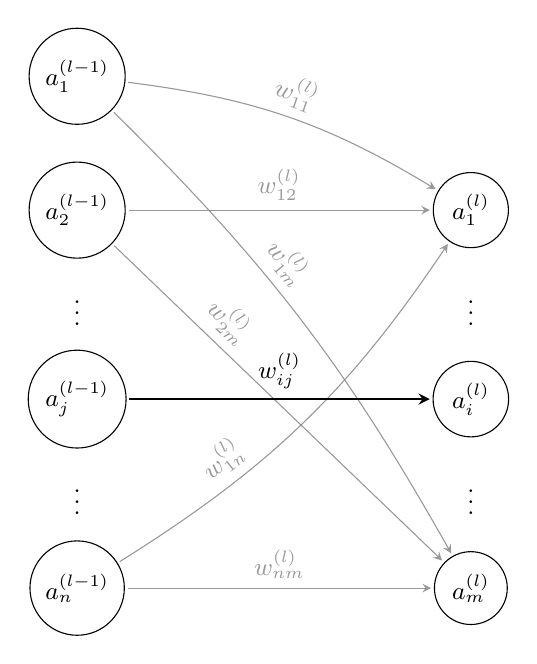
\begin{tikzpicture}[>=stealth, every node/.style={font=\small}, every path/.style={->, shorten >=1pt, shorten <=1pt}]
                % Source layer (l-1) with ellipses to indicate generality
                \node[circle, draw] (N1) at (0,0.5)    {$a_{1}^{(l-1)}$};
                \node[circle, draw] (N2) at (0,-1.2) {$a_{2}^{(l-1)}$};
                \node at (0,-2.4) {$\vdots$};
                \node[circle, draw] (Nj) at (0,-3.6) {$a_{j}^{(l-1)}$};
                \node at (0,-4.8) {$\vdots$};
                \node[circle, draw] (Nn) at (0,-6) {$a_{n}^{(l-1)}$};

                % Target layer l with ellipses
                \node[circle, draw, minimum size=0.9cm] (M1) at (5,-1.2) {$a_{1}^{(l)}$};
                \node at (5,-2.4) {$\vdots$};
                \node[circle, draw, minimum size=0.9cm] (Mi) at (5,-3.6) {$a_{i}^{(l)}$};
                \node at (5,-4.8) {$\vdots$};
                \node[circle, draw, minimum size=0.9cm] (Mm) at (5,-6) {$a_{m}^{(l)}$};

                % faint generic connections to show full connectivity
                \draw[->, gray, opacity=0.8, bend left=12]  (N1) to node[sloped, above] {$w_{11}^{(l)}$} (M1);
                \draw[->, gray, opacity=0.8]                  (N2) to node[sloped, above] {$w_{12}^{(l)}$} (M1);
                \draw[->, gray, opacity=0.8, bend right=12]  (Nn) to node[pos=0.3, sloped, above] {$w_{1n}^{(l)}$} (M1);

                \draw[->, gray, opacity=0.8, bend left=8]   (N1) to node[pos=0.4, sloped, above] {$w_{1m}^{(l)}$} (Mm);
                \draw[->, gray, opacity=0.8]                  (N2) to node[pos=0.30, sloped, above] {$w_{2m}^{(l)}$} (Mm);
                \draw[->, gray, opacity=0.8]   (Nn) to node[sloped, above] {$w_{nm}^{(l)}$} (Mm);

                % highlighted connection showing the general index i,j
                \draw[->, thick] (Nj) to node[midway, above] {$\;w_{ij}^{(l)}\;$} (Mi);
            \end{tikzpicture}
        \end{center}
        \item Each $b_{i}^{(l)}$ is the bias for neuron $i$ in layer $l$.
    \end{itemize}
    The \textbf{gradient} $\nabla E(w)$ then contains the partial derivatives of the loss function with respect to \textbf{each individual weight and bias} in the network:
    \begin{equation}
        \nabla E(w) = \left\{
            \dfrac{\partial \, E}{\partial \, w_{ij}^{(l)}} , \,
            \dfrac{\partial \, E}{\partial \, b_{i}^{(l)}}
        \right\}
    \end{equation}
    The \textbf{core learning rule} still applies, but now we update \textbf{each weight and bias} individually:
    \begin{equation}
        w_{ij}^{(l)} \leftarrow w_{ij}^{(l)} - \eta \,\dfrac{\partial \, E}{\partial \, w_{ij}^{(l)}} \quad \text{and} \quad
        b_{i}^{(l)} \leftarrow b_{i}^{(l)} - \eta \,\dfrac{\partial \, E}{\partial \, b_{i}^{(l)}}
    \end{equation}
    This is how \textbf{gradient descent} is applied in the context of training neural networks.
\end{definitionbox}

\begin{flushleft}
    \textcolor{Green3}{\faIcon{tools} \textbf{How it works (intuitively)}}
\end{flushleft}
Intuitively, gradient descent works as follows:
\begin{enumerate}
    \item Start from an \textbf{initial guess} for the weights $w_{0}$ (often random).
    \item Compute the \textbf{gradient} $\nabla E(w_{0})$ of the loss function at the current weights:
    \begin{equation*}
        \nabla E(w_{0}) = \begin{bmatrix}
            \dfrac{\partial \, E}{\partial \, w_{1}} \\[1.2em]
            \dfrac{\partial \, E}{\partial \, w_{2}} \\[1.2em]
            \vdots \\
            \dfrac{\partial \, E}{\partial \, w_{d}}
        \end{bmatrix}_{w = w_{0}}
    \end{equation*}

    \item Do a step \textbf{against} that gradient to update the weights using the \textbf{core learning rule}:
    \begin{equation*}
        w_{k+1} = w_{k} - \eta \,\nabla E(w_{k})
        \quad \Rightarrow \quad
        w_{1} = w_{0} - \eta \,\nabla E(w_{0})
    \end{equation*}
    Then, the new weights $w_{1}$ should yield a \textbf{lower loss} $E(w_{1}) < E(w_{0})$. If we were on a neural network, we would update \textbf{all weights and biases} similarly:
    \begin{equation*}
        w_{ij}^{(l)} \leftarrow w_{ij}^{(l)} - \eta \,\dfrac{\partial \, E}{\partial \, w_{ij}^{(l)}}
        \quad , \quad
        b_{i}^{(l)} \leftarrow b_{i}^{(l)} - \eta \,\dfrac{\partial \, E}{\partial \, b_{i}^{(l)}}
    \end{equation*}
    \item Repeat until: the gradient becomes small (close to zero), or we reach a maximum number of iterations.
\end{enumerate}

\noindent
\textcolor{Green3}{\faIcon{\speedIcon} \textbf{Convergence Speed}} \textbf{and} \textcolor{Red2}{\faIcon{exclamation-triangle} \textbf{False Positives}}. The speed at which gradient descent converges to the minimum depends on:
\begin{itemize}
    \item The \textbf{shape} of the loss function (e.g., steepness, curvature). It strongly affects how gradient descent behaves:
    \begin{itemize}
        \item \textbf{Convex surface} (like a bowl): Gradient descent always converges there (since there is a \textbf{single global minimum}). However, if $\eta$ is too large, it may oscillate around the minimum.

        \item \textbf{Non-convex surface} (like many hills and valleys): There may be \textbf{multiple local minima} and \textbf{saddle points}. Gradient descent might: 
        \begin{itemize}
            \item[\textcolor{Red2}{\faIcon{exclamation-triangle}}] Get stuck in a \textbf{local minimum} (the derivative is zero, but it is not the global optimum).
            \item Oscillate in flat regions.
            \item Move very slowly along narrow valleys.
        \end{itemize}
    \end{itemize}


    \item The \textbf{learning rate} $\eta$.

    \textcolor{Green3}{\faIcon[regular]{lightbulb}} The \textbf{learning rate} $\eta$ is crucial: it controls \textbf{how big a step} we take each iteration.
    \begin{itemize}
        \item $\eta$ too \textbf{small} $\rightarrow$ \textbf{Learning is very slow} because we take tiny steps (many iterations needed).
        \item $\eta$ too \textbf{large} $\rightarrow$ \textbf{May overshoot the minimum} and even diverge (loss increases instead of decreasing).
        \item Choosing a good $\eta$ is often done via \textbf{experimentation} or using techniques. However, if $\eta$ is chosen well, gradient descent can efficiently find a good set of weights that minimize the loss function.
    \end{itemize}
    Don't worry if this seems abstract now; we'll later learn that \textbf{adaptive optimizers} (like \emph{\textbf{momentum}}, \emph{\textbf{Adam}}, etc.) are more robust ways to handle this.


    \item The \textbf{initial weights} $w_{0}$. In \textbf{convex} functions (like a parabola), there is a global minimum, and \emph{gradient descent} will converge to it. In \textbf{non-convex} functions (like many neural network loss landscapes), there may be multiple local minima, and gradient descent may converge to one of them depending on the starting point. So in practice, we \hl{often run gradient descent multiple times with different initial weights to find a good solution}.
\end{itemize}

\begin{figure}[!htp]
    \centering
    \includegraphics[width=.8\textwidth]{img/learning-and-optimization/convex-bowl-contour.pdf}
    \caption{Example of a \textbf{convex quadratic surface} (bowl-shaped). The contour lines (ellipses) represent levels of constant error $E\left(w_{1}, w_{2}\right)$. There is a \textbf{single global minimum} at the center of the bowl ($w_{1}^{*} = 2, w_{2}^{*} = -1$), and outer ellipses represent higher error values. This is the ideal scenario for gradient descent, as it will always converge to the global minimum regardless of the starting point (similar to Figure \ref{fig:error-geometric-interpretation-1}, page \pageref{fig:error-geometric-interpretation-1}).}
    \label{fig:convex-bowl-contour}
\end{figure}

\begin{figure}[!htp]
    \centering
    \includegraphics[width=\textwidth]{img/learning-and-optimization/non-convex-wavy-contour.pdf}
    \caption{Example of a \textbf{non-convex surface} with multiple local minima and saddle points. The loss function $E\left(w_{1}, w_{2}\right)$ has two components: (1) the \textbf{quadratic bowl} that pushes weights toward the global minimum, and (2) the \textbf{sinusoidal term} that introduces \emph{oscillations} in the surface. Those oscillations create \textbf{small waves} (bumps and dips). Each dip (a small valley) is a \emph{local minimum}, and each bump is a \emph{local maximum} or ridge. This is what happens in \textbf{non-linear models} like deep neural networks, where the composition of many layers and activations makes the error surface very complex (and non-convex). There are thousands or millions of such local minima, making optimization challenging. Gradient descent may get trapped in one of these local minima instead of finding the global minimum. However, in practice, many local minima have \textbf{similar performance}, so this isn't always bad.}
    \label{fig:non-convex-surface-contour}
\end{figure}